% Initialisation
\documentclass[
	fontsize=11pt
	headlines=2,
	footlines=2,
	parskip=half
]{scrartcl}

\usepackage[left=2.54cm,top=2.54cm,right=2.54cm,bottom=2.54cm,headheight=30pt]{geometry}

% Enforce UTF8 encoding
\usepackage[utf8]{inputenc}

% Colours
\usepackage[dvipsnames]{xcolor}

% Header and footer
\usepackage{scrlayer-scrpage}
\ohead{SENG4800 - Individual interim report \\ \today}
\cfoot{\pagemark}

% Document title and author
\title{3D visualisation of large data in a multi-platform environment}
\author{Monica Olejniczak}

% Sections
\setcounter{secnumdepth}{4}
\setcounter{tocdepth}{4}
\usepackage[compact]{titlesec}
%\titlespacing{\paragraph}{0pt}{*0}{8pt}

% http://tex.stackexchange.com/questions/198830/section-title-with-runin-and-koma-class

% Abstract
\usepackage{abstract}
\setlength{\absleftindent}{0pt}
\setlength{\absrightindent}{0pt}
\renewcommand{\absnamepos}{flushleft}
\renewcommand{\abstractnamefont}{\normalfont\Large\bfseries}

% Table of contents
\usepackage[nottoc,numbib]{tocbibind}

% Links
\usepackage{hyperref}

% Todo notes
\usepackage{todonotes}
\presetkeys{todonotes}{inline}{}

% Gantt charts
\usepackage{pgfgantt}

% Tables
\usepackage{booktabs}
\usepackage{tabularx}
\renewcommand{\arraystretch}{1.5}
\setlength{\textfloatsep}{0.1em}

% Additional
\usepackage{float}
\usepackage{spreadtab}
\usepackage{etoolbox}
\usepackage{multicol}
\usepackage{caption} 
\usepackage{subcaption}
% Remove spacing before and after captions
\captionsetup[table]{aboveskip=-8pt}
\captionsetup[table]{belowskip=8pt}
\captionsetup[figure]{belowskip=-15pt}
% Remove indentation on description lists
\usepackage{enumitem}
\setlist[description, 1]{leftmargin=0pt}
\setlist[description, 2]{wide=20pt}

% References
\usepackage[numbers]{natbib}
% Left align text
\renewcommand*{\bibfont}{\raggedright}

% Appendices
\usepackage[toc,page]{appendix}

% Commands
\newcommand{\rating}[1]{
	\ifnumless{#1}{20 * 100} {Very low} {
		\ifnumless{#1}{40 * 100} {Low} {
			\ifnumless{#1}{60 * 100} {Medium} {
				\ifnumless{#1}{80 * 100} {High} {
					Very high
				}
           	}
		}
	}
}

\begin{document}

	\vspace*{\fill}
	% Title page
	\makeatletter
	\begin{center}
		\Huge\textbf{\textsf{\@title}}
		\vspace{0.5em}\\
		\Large\textbf{\textsf{\@author}}
	\end{center}
	\makeatother
	
	\begin{abstract}
		\todo{Data visualisation is the presentation of data in a visual context and is particularly important in data analytics since humans are able to recognise patterns, trends and correlations more easily \citep{grinstein2002introduction}.
		
		This project aims to develop touch-based visualisations in three-dimensions and will focus on using large data in a generic way to demonstrate general applicability. The visualisations will provide touch-capability so they are able to be viewed on a smart device.}
	\end{abstract}
	\vspace*{\fill}
	
	\newpage
	\tableofcontents
	\newpage
	
	\section{Introduction} {
	\label{sec:introduction}
		
		Data visualisation is the presentation of information in a visual context. It is particularly important in data analytics, since humans are able to recognise patterns, trends and correlations more easily \citep{grinstein2002introduction}. Recognising these relationships is critical when working with big data, as the mass of information needs to be filtered and interpreted, so analysts can make informed decisions \citep{hendley1995case}. This task can be resolved by creating effective data visualisations, as they have the potential to lead to analytic discovery or be used for data reduction \citep{rohrer1997web}. Analytic discovery highlights important information in large volumes of data, while data reduction removes uninteresting information so a tool can be applied to the remaining data.
		
		This research presents the main issues and challenges associated with big data and its characteristics, discusses how to visualise information and delves into effective visualisation techniques that can be applied with big data. The rest of this report outlines the details of this project which include its goals, plan for development and schedule. This report concludes with the ethical issues that arise from developing this project.
		
		\subsection{Big data} {
		
			Big data can be defined as the amount of information stored, managed and processed just beyond the capability of present technology \citep{kaisler2013big}.
			
			\subsubsection{Characteristics} {
			
				\begin{table}[H]
				\caption{The various characteristics of big data.}
				\begin{tabularx}{\textwidth}{@{}lX@{}}
					\toprule
					\textbf{Name} & \textbf{Description} \\
					\midrule
					Volume & This is the quantity of data that is available to an organisation \citep{kaisler2013big} and can exist in the size of petabytes \citep{katal2013big}. \\
					Velocity & Data velocity measures the rate of which data is created \citep{ferguson2012architecting} and how fast it is generated and processed from various sources \citep{katal2013big}. \\
					Variety & Refers to various forms of data and could consist of raw, structured, semi-structured or unstructured data \citep{ferguson2012architecting} such as text, email, image or video. \\
					Variability & The inconsistencies of the data flow \citep{katal2013big} which can effect data maintainability. \\
					Value & This refers to the usefulness of data in making decisions \citep{kaisler2013big}. \\
					Complexity & The degree of how much the data is linked, connected and correlated. Changes that are made to a few elements can either have a substantial, or no effect, on the system based on this characteristic \citep{kaisler2013big}. \\
					\bottomrule
				\end{tabularx}
				\end{table}
			
			}
			
			\subsubsection{Issues and challenges} {
				
				\paragraph{Storage and transport} {
				
					There are rigorous demands placed on storage, networks and servers when data is being produced by almost everything \citep{katal2013big}. Uploading data to the cloud is an option \citep{katal2013big} \citep{labrinidis2012challenges}, but may not be feasible for real-time applications due to its upload time \citep{katal2013big}. 
					
					\citet{kaisler2013big} discusses that transporting big data is difficult due to hardware and network constraints. They calculated that it would take approximately 2800 hours to transfer an exabyte of data with a reliable network connection, which is substantially longer than processing it.
				
				}

				\paragraph{Processing} {
				
					\citet{labrinidis2012challenges} mention that processing a large volume of data takes a significant amount of time to analyse. This is especially due to data volumes increasing more rapidly than the computing resources available \citep{katal2013big}, which is a cause for concern. It is not feasible to scan an entire data set to locate suitable elements. To effectively process big data, either parallel processing \citep{kaisler2013big}, or data indexing during collection and storage \citep{katal2013big} \citep{labrinidis2012challenges}, needs to take place. However, index structures are usually designed to only support a few classes of search criteria and are challenging to design when the data volume grows rapidly \citep{labrinidis2012challenges}.
					
					Hard disk drives are being increasingly replaced by solid state drives and other technologies due to their processing limitations. This has several implications in data processing, which includes query processing, algorithms, query scheduling, database design, concurrency control methods and recovery methods \citep{labrinidis2012challenges}.
					
				}
				
				\paragraph{Privacy and security} {
				
					The privacy and security of data is a primary concern for big data. It raises ethical issues which have been mentioned in Section~\ref{sec:personal_data} and can be considered a technical and sociological problem. Strict laws and regulations can be enforced on certain types of data, which govern what can be done with that information \citep{labrinidis2012challenges}. 
					
					Users are often unaware of the information that has been collected from them \citep{katal2013big} and often fear the potential misuse of their personal data, especially when it has been linked from multiple sources \citep{labrinidis2012challenges}. This is particularly problematic when users wish to remain anonymous and unidentifiable.
					
				}
				
			}
				
			\subsubsection{Importance} {			
	
			}
		
		}
		
		\subsection{Information visualisation} {
		
			The creation of an effective visualisation requires finding an appropriate visual mapping for a specific task \citep{rohrer1997web}. This may prove to be difficult as there are a large array of visualisations that could be applied to a given data set. Moreover, \citet{hendley1995case} discusses that a 3-dimensional representation of data provides a rich user experience, due to the increased information density, as opposed to the traditional 2-dimensional representation. 
		
		}
		
		\subsection{Effective visualisation techniques/Visualising big data} {
		
		}
	
	}
	
	\newpage
	
	\section{Project plan} {
	\label{sec:project_plan}
		
		This project will be developed in a web environment to ensure the creation of a platform independent system. It will primarily use \href{http://threejs.org/}{Three.js}, a JavaScript library that abstracts WebGL, as a tool for creating 3D visualisations. An initial prototype was designed and has been discussed in Appendix~\ref{app:current_progress}. The main \emph{goals} of this project are to:
		
		%\begin{multicols}{2}
		\begin{itemize}
			\item Visualise big data in a time efficient manner.
			\begin{itemize}
				\item This should be a reasonable loading time for the user.
			\end{itemize}
			\item Ensure the visualisation is aesthetically pleasing and of high quality.
			\item Apply the visualisations to multiple datasets and ensure they are scalable. 
			\item Integrate the results into the group project.
			\begin{itemize}
				\item Apply the visualisations in different ways.
			\end{itemize}
			\item Learn how 3D visualisations can effectively convey information.
			\item Learn how to optimise calls and understand what drains processing resources easily.
			\begin{itemize}
				\item This can be measured with a \href{http://jsperf.com/}{JavaScript performance testing environment}.
			\end{itemize}
		\end{itemize}
		%\end{multicols}
		
		To facilitate these goals, this project will involve creating visualisations that are able to compared with one another. This will be done so it can be seen which visualisation is more effective at representing a dataset in particular applications. With this in mind, it has been decided that heat maps will be used as the basis of this project as they have a wide array of applications. Figure~\ref{fig:heat_maps} features two different ways of visualising a heat map. It has potential applications in displaying a 3D column or bar chart, financial and geographical data. It is interesting to note that geographical data can be applied to both visualisations, where the image on the left can be mapped to a sphere and could represent population data, while the other could represent pollution levels in a city.
		
		\begin{figure}[H]
			\centering
			\begin{subfigure}[b]{0.4\textwidth}
                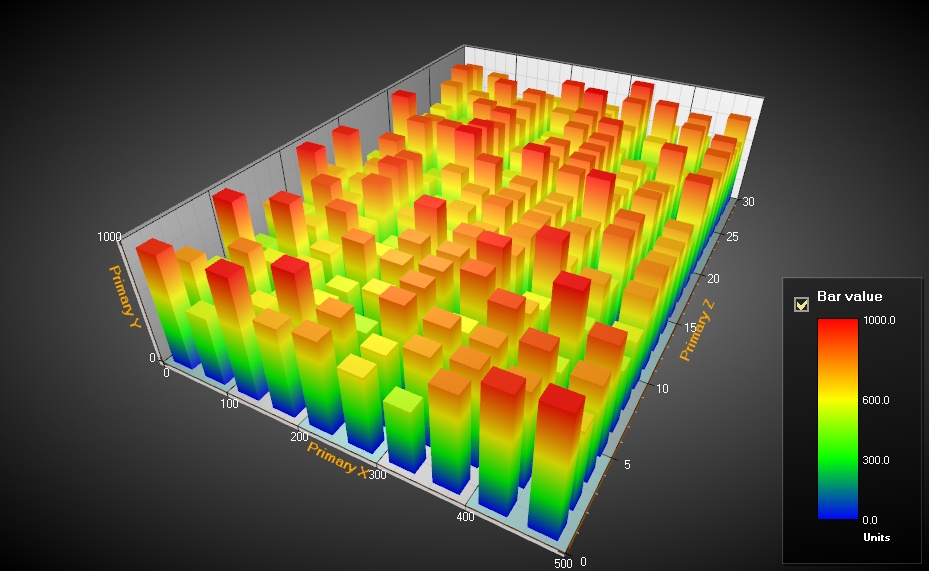
\includegraphics[width=\textwidth,height=3.5cm]{images/heat-map-1}
	        \end{subfigure}
	        \begin{subfigure}[b]{0.4\textwidth}
                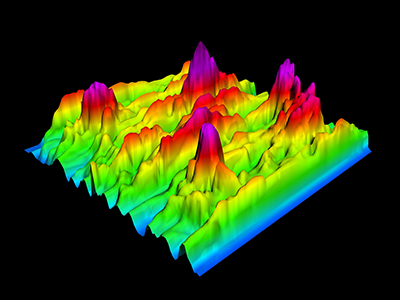
\includegraphics[width=\textwidth,height=3.5cm]{images/heat-map-2}
	        \end{subfigure}
			\caption{Two different representations of a heat map \citep{tuomainen2014financial} \citep{fuchs2006physiological}.}
			\label{fig:heat_maps}
		\end{figure}
		
		The data for the visualisations can easily be represented as a flat array. It may or may not need to be preprocessed, as this depends on the format of the data. This data representation has also been adopted by \href{https://www.chromeexperiments.com/globe}{The WebGL Globe} Chrome Experiment, as shown in Appendix~\ref{app:globe}, is a great example of visualising big data in an efficient way. This open platform project clearly demonstrates that the goals of this project are achievable. They encourage users to use their own datasets, ensuring a certain level of scalability and applications with geographical data.
		
		The development of these visualisations will involve using the established \href{http://threejs.org/docs/#Reference/Extras.Geometries/BoxGeometry}{BoxGeometry} and NURBS surface that are available in Three.js. The \href{http://threejs.org/examples/webgl_geometry_nurbs.html}{NURBS example}, as displayed in Appendix~\ref{app:nurbs}, proves that it is possible to render a smooth 3D surface. This can be applied to represent a heat map and if there lie difficulties in implementing this, then an simpler representation can be modelled.
		
		\subsection{Stakeholders} {
		\label{sec:stakeholders}

			\begin{itemize}
				\item The users of the project.
				\item Researchers interested in visualising big data.
				\item University of Newcastle.
				\item School of Engineering and Computer Science.
				\begin{itemize}
					\item Dr. Shamus Smith.
					\item Members of the Software Engineering \emph{(Honours)} Final Year Project.
				\end{itemize}
				\item School of Nursing and Midwifery.
				\begin{multicols}{3}
				\begin{itemize}
					\item Prof. Sally Chan.
					\item Dr. Sharyn Hunter.
					\item Dr. Amanda Wilson.
				\end{itemize}
				\end{multicols}
			\end{itemize}		
		
		}
		
		\subsection{Scope} {
		\label{sec:scope}
		
			\subsubsection{Inclusions and exclusions} {
			\label{sec:inclusions_and_exclusions}
			
				\begin{table}[H]
				\caption{A list of what will and will not be included in this project.}
				\begin{tabularx}{\textwidth}{@{}XX@{}}
					\toprule
					\textbf{Inclusions} & \textbf{Exclusions} \\
					\midrule
					3D visualisations that can be compared. & 2D visualisations. \\
					Basic interaction - pan, zoom and rotate. & Advanced touch interactions. \\
					Data filtering. & Volume selection. \\
					Data integration with the Final Year Project. & \\
					\bottomrule
				\end{tabularx}
				\end{table}
			
			}
		
		}
		
		\subsection{Dependencies} {
		\label{sec:dependencies}
		
			\begin{table}[H]
			\caption{A list of project dependencies.}
			\begin{tabularx}{\textwidth}{@{}XX@{}}
				\toprule
				\textbf{Dependency} & \textbf{Description} \\
				\midrule
				BitBucket & Source code host \\
				SourceTree & Git client \\
				Node.js & Runtime environment \\
				Three.js & WebGL abstraction \\
				RequireJS & Dependency injection \\
				LaTeX & Typesetting \\
				Shamus Smith & Project supervisor \\
				\bottomrule
			\end{tabularx}
			\end{table}
		
		}
		
		\subsection{Constraints} {
		\label{sec:constraints}
			
			\begin{itemize}
				\item The final deliverables have a non-negotiable deadline.
				\item There is a limited amount of hours that can be contributed to the project per week.
				\item There is no allocated budget for this project.
				\begin{itemize}
					\item Resources cannot be easily purchased to upgrade processing hardware.
				\end{itemize}
				\item The choice of platform may not be fast enough to process big data.
			\end{itemize}
		
		}
		
		\subsection{Assumptions} {
		\label{sec:assumptions}
			
			%\begin{multicols}{2}
			\begin{itemize}
				\item There will be adequate time to develop the project.
				\item The project supervisor will be available when required and is able to offer sufficient guidance.
				\item Project deliverables are reviewed and approved by the project supervisor within a specified time frame.
				\item The project scope, requirements and assessment deadlines will not change.
				\item The hardware used to develop the project will remain functional over the course of the year.
				\item The risks for the project have been identified and accounted for.
			\end{itemize}
			%\end{multicols}
		
		}
		
		\subsection{Risks} {
		\label{sec:risks}

			The following table outlines the risks involved in this project. A more detailed risk assessment can be found in Appendix~\ref{app:risk_assessment}.
			
			\begin{table}[H]
			\caption{The list of risks associated with this project and their appropriate mitigation strategies.}
			\begin{tabularx}{\textwidth}{@{}lp{0.35\linewidth}X@{}}
				\toprule
				\textbf{Id} & \textbf{Description} & \textbf{Strategy} \\
				\midrule
				1 & Deliverables are not completed by the deadline. & \emph{Reduction:} Adhere to the project schedule. \\
				2 & Hardware failure. & \emph{Reduction:} Hardware will be treated with care. \\
				3 & Hardware cannot efficiently process big data. & \emph{Reduction:} Make optimisations where possible. \\
				4 & Software platform cannot efficiently process big data. & \emph{Reduction and acceptance:} Determine what is considered big data for this platform to minimise risk. \\
				5 & Scope is too large. & \emph{Reduction:} Reasonable requirements are established in the proposal with the project supervisor. \\
				6 & Code is lost. & \emph{Reduction:} Version control is used with small commits to minimise the impact of loss. \\
				7 & Project cannot be integrated to the group project. & \emph{Reduction:} Allocate enough time to this and contribute to the group through other means. \\
				8 & Project is not useful or applicable to the group. & \emph{Reduction and acceptance} Discuss and confirm applicability with the group and project supervisor before commencing. Alter the visualisation when required. \\
				\bottomrule
			\end{tabularx}
			\end{table}
		
		}
	
	}
	
	\newpage
	
	\section{Project schedule} {
	\label{sec:project_schedule}
	
		The project plan, which was outlined in Section~\ref{sec:project_plan}, is to be completed according to the project schedule. This has been demonstrated through the Gantt chart in Figure~\ref{gantt:schedule} below, and clearly highlights each milestone that is critical to the success of this project. These include:
		
		\begin{description}
			\item[Progress reports:] Progress update meetings have been scheduled with the project supervisor on a fortnightly basis.
			\item[Individual research presentation:] The presentation requires written preparation and rehearsal. It should be completed by the end of the first week so more important tasks can be focused on.
			\item[Final report:] This report encompasses the deliverables of the project as they form the basis for the documentation. The report will need to be allocated at least one fortnight after the deliverables have been completed, so it can be completed to a good standard of quality.
			\begin{description}
				\item[Basic deliverables:] This should be completed in two weeks and consists of the implementation for a single visualisation and interactions for panning, zooming and rotating.
				\item[Intermediate deliverables:] These deliverables have been designated one month to complete. It includes the ability to filter data, apply the visualisation to one or more large datasets and the implementation of another visualisation.
				\item[Advanced deliverables:] This has also been allotted one month to complete and it is a core requirement to integrate the data to the group project. Analysing the computational power and the scalability of the visualisations are considered to be more important than the other tasks and thus have been allocated more time.
			\end{description}
		\end{description}
		
		Unfortunately, it is quite probable that no work will be undertaken towards the individual project during the mid-year recess. This is due to the need to prepare for and attend RoboCup 2015, China. It has therefore been omitted from the schedule.
        
		\begin{figure}[H]
	        \resizebox{\textwidth}{!}{\begin{ganttchart}[
	vgrid={*6{black, dotted},*1{black, dashed}},
	x unit=0.3cm,
	y unit title=0.75cm,
	y unit chart=1cm,
	time slot format=isodate,
	title height = 1,
	title/.append style={draw=none, fill=RoyalBlue!40!black},
	title label font=\sffamily\bfseries\color{white},
	title label node/.append style={below=-1.6ex},
	title left shift=.05,
	title right shift=-.05,
	title top shift=.05,
	title height=.95,
	bar/.append style={draw=none, fill=MidnightBlue!75},
	bar height=.6,
	bar label font=\normalsize\color{black!80},
%	group right shift=0,
%	group top shift=.6,
%	group height=.3,
%	group peaks height=.2,
%	bar incomplete/.append style={fill=red}
]
{2015-07-27}{2015-11-08} % start and end date

\newganttchartelement{optionalbar}{
	optionalbar/.style={
		shape=rectangle,
		fill=black!70
	},
	optionalbar height=.6
}

\gantttitle{Semester 2}{105} \ganttnewline
\gantttitlecalendar*{2015-07-27}{2015-11-08}{month=name} \ganttnewline
\gantttitlecalendar*{2015-07-27}{2015-09-20}{week=1}
\gantttitle{Recess}{14}
\gantttitlecalendar*{2015-10-05}{2015-11-08}{week=9}

% Progress reports
\ganttnewline \ganttgroup{Meetings}{2015-07-28}{2015-11-04}

	% Group meetings
	\ganttnewline \ganttbar{Group}{2015-07-28}{2015-07-28}
	\ganttbar{}{2015-08-04}{2015-08-04}
	\ganttbar{}{2015-08-11}{2015-08-11}
	\ganttbar{}{2015-08-18}{2015-08-18}
	\ganttbar{}{2015-08-25}{2015-08-25}
	\ganttbar{}{2015-09-01}{2015-09-01}
	\ganttbar{}{2015-09-08}{2015-09-08}
	\ganttbar{}{2015-09-15}{2015-09-15}
	\ganttbar{}{2015-10-06}{2015-10-06}
	\ganttbar{}{2015-10-13}{2015-10-13}
	\ganttbar{}{2015-10-20}{2015-10-20}
	\ganttbar{}{2015-10-27}{2015-10-27}
	\ganttbar{}{2015-11-03}{2015-11-03}

	% Supervisor meetings
	\ganttnewline \ganttbar{Supervisor}{2015-07-28}{2015-07-28}
	\ganttbar{}{2015-08-11}{2015-08-11}
	\ganttbar{}{2015-08-25}{2015-08-25}
	\ganttbar{}{2015-09-08}{2015-09-08}
	\ganttbar{}{2015-10-06}{2015-10-06}
	\ganttbar{}{2015-10-20}{2015-10-20}
	\ganttbar{}{2015-11-03}{2015-11-03}

	% Client meetings
	\ganttnewline \ganttbar{Client}{2015-08-05}{2015-08-05}
	\ganttbar{}{2015-08-26}{2015-08-26}
	\ganttbar{}{2015-10-07}{2015-10-07}
	\ganttbar{}{2015-10-21}{2015-10-21}

% Group participation
\ganttnewline \ganttgroup{Group participation}{2015-07-27}{2015-11-06}

	% Overall work
	\ganttnewline \ganttbar{Work}{2015-07-27}{2015-11-06}

	% Progress reports
	\ganttnewline \ganttbar{Progress reports}{2015-07-31}{2015-07-31}
	\ganttbar{}{2015-08-07}{2015-08-07}
	\ganttbar{}{2015-08-14}{2015-08-14}
	\ganttbar{}{2015-08-21}{2015-08-21}
	\ganttbar{}{2015-08-28}{2015-08-28}
	\ganttbar{}{2015-09-04}{2015-09-04}
	\ganttbar{}{2015-09-11}{2015-09-11}
	\ganttbar{}{2015-09-18}{2015-09-18}
	\ganttbar{}{2015-10-09}{2015-10-09}
	\ganttbar{}{2015-10-16}{2015-10-16}
	\ganttbar{}{2015-10-23}{2015-10-23}
	\ganttbar{}{2015-10-30}{2015-10-30}

	% Group system demonstration - week 10
	\ganttnewline \ganttgroup{Group system demonstration}{2015-10-06}{2015-10-14}
	\ganttnewline \ganttbar{Preparation}{2015-10-06}{2015-10-14}

	% Group final report - week 12
	\ganttnewline \ganttgroup{Group final report}{2015-10-20}{2015-10-30}
	\ganttnewline \ganttbar{Preparation}{2015-10-20}{2015-10-20}
	\ganttbar{}{2015-10-27}{2015-10-27}
	\ganttnewline \ganttbar{Document}{2015-10-23}{2015-10-30}

	% Open day presentation - week 13
	\ganttnewline \ganttgroup{Open day presentation}{2015-10-30}{2015-11-04}
	\ganttnewline \ganttbar{Preparation}{2015-10-30}{2015-11-04}

% Individual work
\ganttnewline \ganttgroup{Individual work}{2015-07-27}{2015-11-06}

	% Individual research presentation - week 1
	\ganttnewline \ganttgroup{Presentation}{2015-07-27}{2015-07-31}
	\ganttnewline \ganttbar{Preparation}{2015-07-27}{2015-07-31}
	\ganttnewline \ganttbar{Rehearsal}{2015-07-30}{2015-07-31}

	% Individual final report - week 13
	\ganttnewline \ganttgroup{Individual final report}{2015-08-01}{2015-11-06}
	\ganttnewline \ganttbar{Summarise basic deliverables}{2015-08-22}{2015-08-24}
	\ganttnewline \ganttbar{Summarise intermediate deliverables}{2015-09-24}{2015-09-26}
	\ganttnewline \ganttbar{Summarise advanced deliverables}{2015-10-23}{2015-10-25}
	\ganttnewline \ganttbar{Finalise}{2015-10-23}{2015-11-06}

		% Basic deliverables
		\ganttnewline \ganttgroup{Basic deliverables}{2015-08-01}{2015-08-21}
		\ganttnewline \ganttbar{Implementation (1)}{2015-08-01}{2015-08-21}
		\ganttnewline \ganttbar{Basic interaction}{2015-08-16}{2015-08-21}

		% Intermediate deliverables
		\ganttnewline \ganttgroup{Intermediate deliverables}{2015-08-22}{2015-09-23}
		\ganttnewline \ganttbar{Data filtering}{2015-08-22}{2015-09-16}
		\ganttnewline \ganttbar{Implementation (2)}{2015-08-26}{2015-09-23}
		\ganttnewline \ganttbar{Apply datasets}{2015-09-9}{2015-09-23}

		% Advanced deliverables
		\ganttnewline \ganttgroup{Advanced deliverables}{2015-09-24}{2015-10-22}
		\ganttnewline \ganttbar{Integrate data}{2015-09-24}{2015-10-22}
		\ganttnewline \ganttoptionalbar{Benchmark scalability}{2015-10-01}{2015-10-22}
		\ganttnewline \ganttoptionalbar{Analyse computational power}{2015-10-01}{2015-10-22}
		\ganttnewline \ganttoptionalbar{Perform user study}{2015-10-15}{2015-10-22}
		\ganttnewline \ganttoptionalbar{Port to a touch-interface}{2015-10-15}{2015-10-22}
		\ganttnewline \ganttoptionalbar{Incorporate touch gestures}{2015-10-15}{2015-10-22}

% % Examples of gantt chart capabilities: 
% \ganttnewline \ganttgroup{Label Text}{2015-08-20}{2015-10-5}
% \ganttnewline \ganttmilestone{Label Text}{2015-08-3}
% \ganttnewline \completedganttbar{Label Text}{2015-8-9}{2015-8-13}
% \ganttnewline \ganttlinkedmilestone{Label Text}{2015-08-19}
% \ganttnewline \ganttbar{Label Text}{2015-09-11}{2015-10-5}
% \ganttnewline \optionalganttbar{Label Text}{2015-10-6}{2015-10-26}

\end{ganttchart}
}
			\caption[Project schedule] {A Gantt chart illustrating the project schedule. Grey bars indicate optional tasks.}
			\label{gantt:schedule}
		\end{figure}
		
	}
	
	\newpage
	
	\section{Ethical issues} {
	\label{sec:ethical_issues}
		
		The data used to model the visualisations have the potential to lead to ethical issues by containing personal data or copyrighted information.
		
		\subsection{Personal data} {
		\label{sec:personal_data}
		
			Personal data is information that is able to identify a person and could be obtained when this project is integrated with the final year group project. It is necessary to log user information in order to obtain the data required to display the visualisations. Users must:
			
			\begin{itemize}
				\item Remain informed of how the data is stored, preserved and used. 
				\item Consent to the storage of this information.
				\item Be informed of how confidentiality will be maintained.
			\end{itemize}
			
			The research data should be anonymised, to increase confidentiality, so individuals cannot be identified from the data. This can be achieved by recording different users with an arbitrary value such as a colour or unique identifier, instead of their name or student number. It is also feasible to not record this data at all and simply just store the values associated with their touches.
		
		}
		
		\subsection{Copyrighted information} {
		\label{sec:copyright}
		
			This poses as an issue when the data used for the visualisation is extracted from an external source. The data should be under a public copyright licence to ensure that there are no copyright infringements when applying it to the project.
			
			A possible solution to this issue is to instead generate fake data. This will see the benefit of viewing the visualisation under a large dataset, removing any concern over copyright issues. However, the visualisation will not display real information and the generated data may appear too random. This data could be generated within a program or by using free online tools.
		
		}
	
	}
	
	\newpage

	\bibliographystyle{plainnat}
	\bibliography{references}
	
	\newpage
	
	\begin{appendices}
	
		\section{Current progress} {
		\label{app:current_progress}
		
			Initially, this project was inspired by the visualisation of flight paths as shown in Figure~\ref{fig:flight_paths}. These flight paths could instead represent touch-gestures that could be integrated into the group project. A proof of concept of this visualisation was developed to test the capabilities of the Three.js library.
			
			\begin{figure}[H]
        		\href{http://nats.aero/blog/2014/03/europe-24-air-traffic-data-visualisation/}{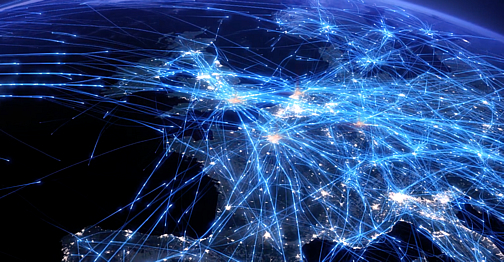
\includegraphics[width=\textwidth]{images/flight-paths}}
				\caption{Air traffic data visualisation \citep{nats2014air}.}
				\label{fig:flight_paths}
			\end{figure}
			
			The format of the data needed to be confirmed before generating it. To do this, a test runner was created to evaluate any performance differences in reading and parsing array data as opposed to objects. The results of this test, which are demonstrated in Figure~\ref{fig:performance_test}, conclude that reading and parsing array data is far more efficient.
			
			\begin{figure}[H]
        		\href{http://jsperf.com/object-and-array-reading}{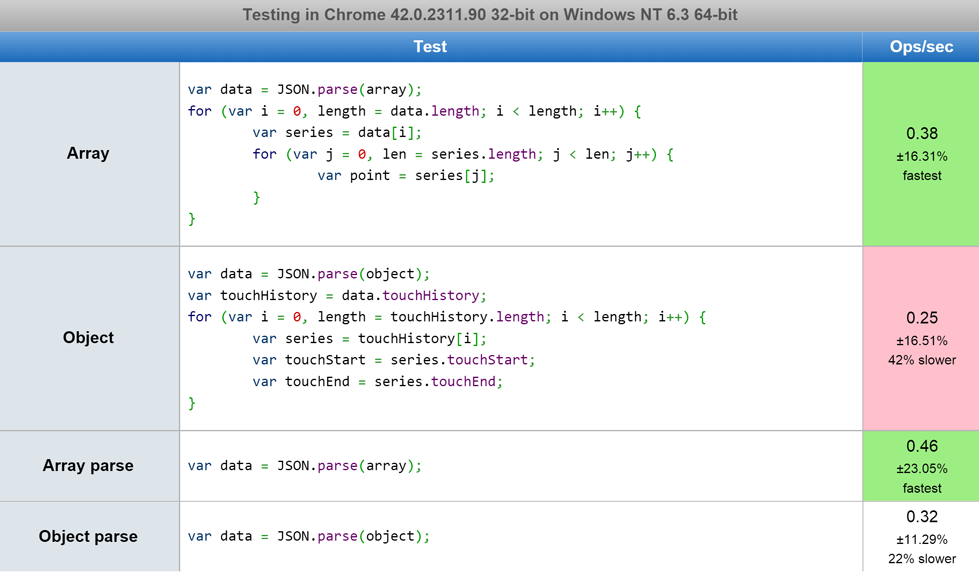
\includegraphics[width=\textwidth,height=8.5cm]{images/performance-test}}
				\caption{The results of the performance test.}
				\label{fig:performance_test}
			\end{figure}
			
			Lines are incredibly difficult to draw in WebGL \citep{deslauriers2015lines} and was the first challenge when attempting to develop this visualisation. There are two main methods of rendering a line using the Three.js library: 
			
			\begin{description}
				\item[Line Object:] The default thickness of the line is too thin to highlight intersections with alpha blending. To resolve this, the \emph{lineWidth} property should be used. However, it is not supported in Windows which limits the availability of the system.
				\item[TubeGeometry:] This geometry does not render acute angles accurately and results in a thinner and deformed tube structure. It also does not shade intersecting tubes correctly, which is highlighted in Figure~\ref{fig:tube_geometry}. While the code could be modified through a pull request, this would be too time consuming as the mathematics behind it is very complex and would need to be learned.
			\end{description}
			
			\begin{figure}[H]
        		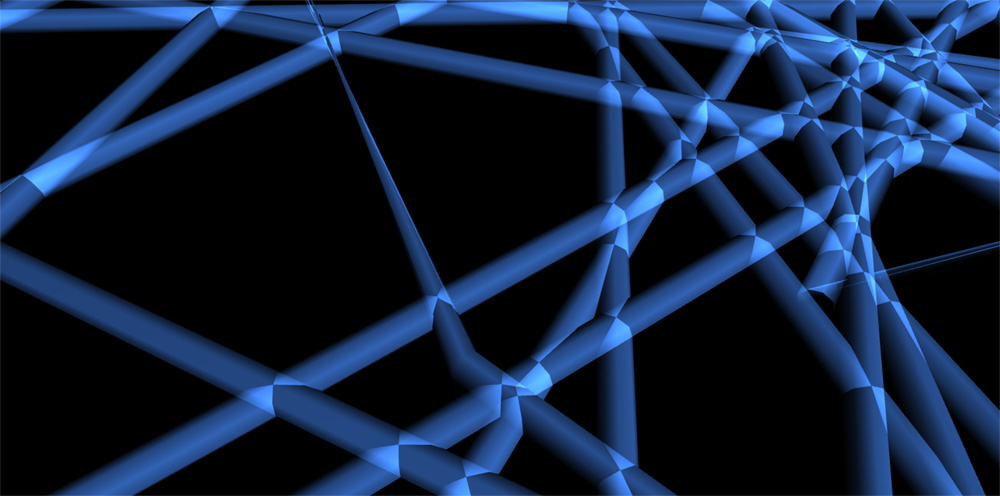
\includegraphics[width=\textwidth]{images/tube-geometry}
				\caption{The issues with TubeGeometry.}
				\label{fig:tube_geometry}
			\end{figure}
			
			The visualisation did provide relatively good results which have been presented in Figure~\ref{fig:proof_of_concept}. However, when closely inspected the issues with its finer details were too prominent. Given the difficulty of amending the issues that arise when rendering a line, this idea was scrapped.
			
			\begin{figure}[H]
        		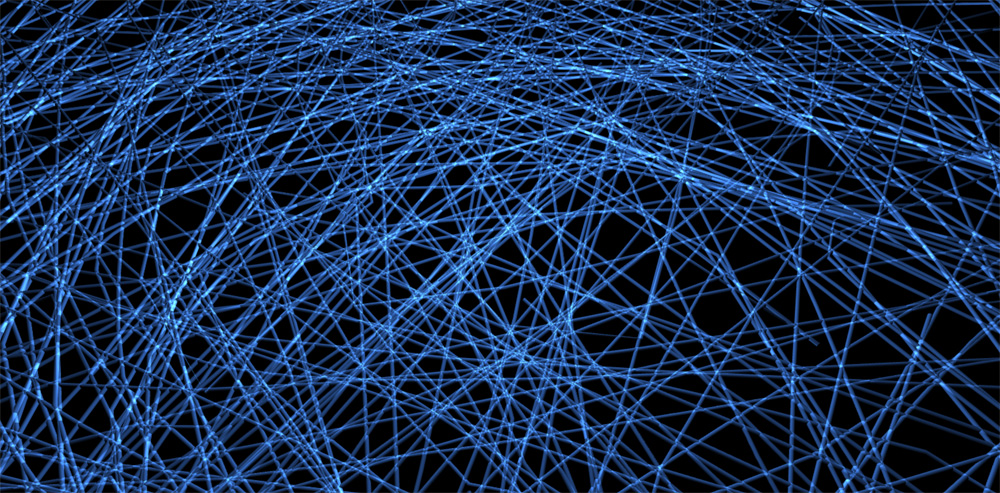
\includegraphics[width=\textwidth]{images/proof-of-concept}
				\caption{An example of the visualisation that was developed.}
				\label{fig:proof_of_concept}
			\end{figure}
		
		}
		
		\newpage
	
		\section{Examples} {
		\label{app:examples}
		
			\subsection{WebGL Globe} {
			\label{app:globe}
		
				\begin{figure}[H]
        			\href{https://www.chromeexperiments.com/globe}{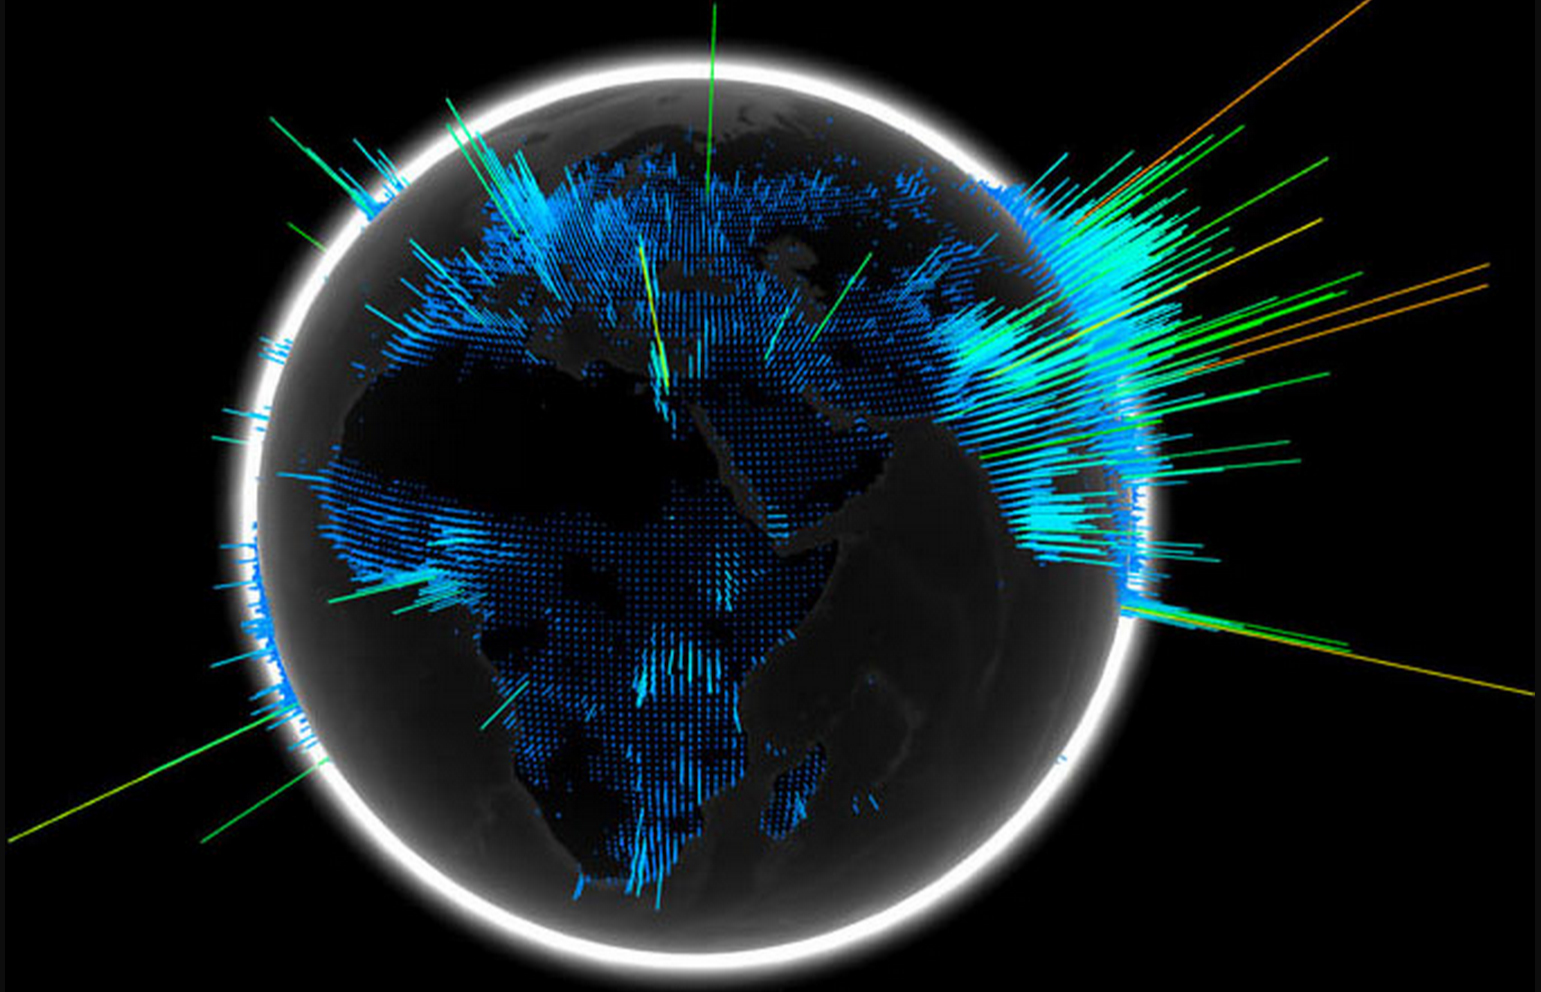
\includegraphics[width=\textwidth]{images/globe}}
					\caption{A screenshot of the WebGL Globe representing population data \citep{google2011globe}.}
					\label{fig:webgl_globe}
				\end{figure}
		
			}
		
			\subsection{NURBS curve and surface} {
			\label{app:nurbs}		
		
				\begin{figure}[H]
        			\href{http://threejs.org/examples/webgl_geometry_nurbs.html}{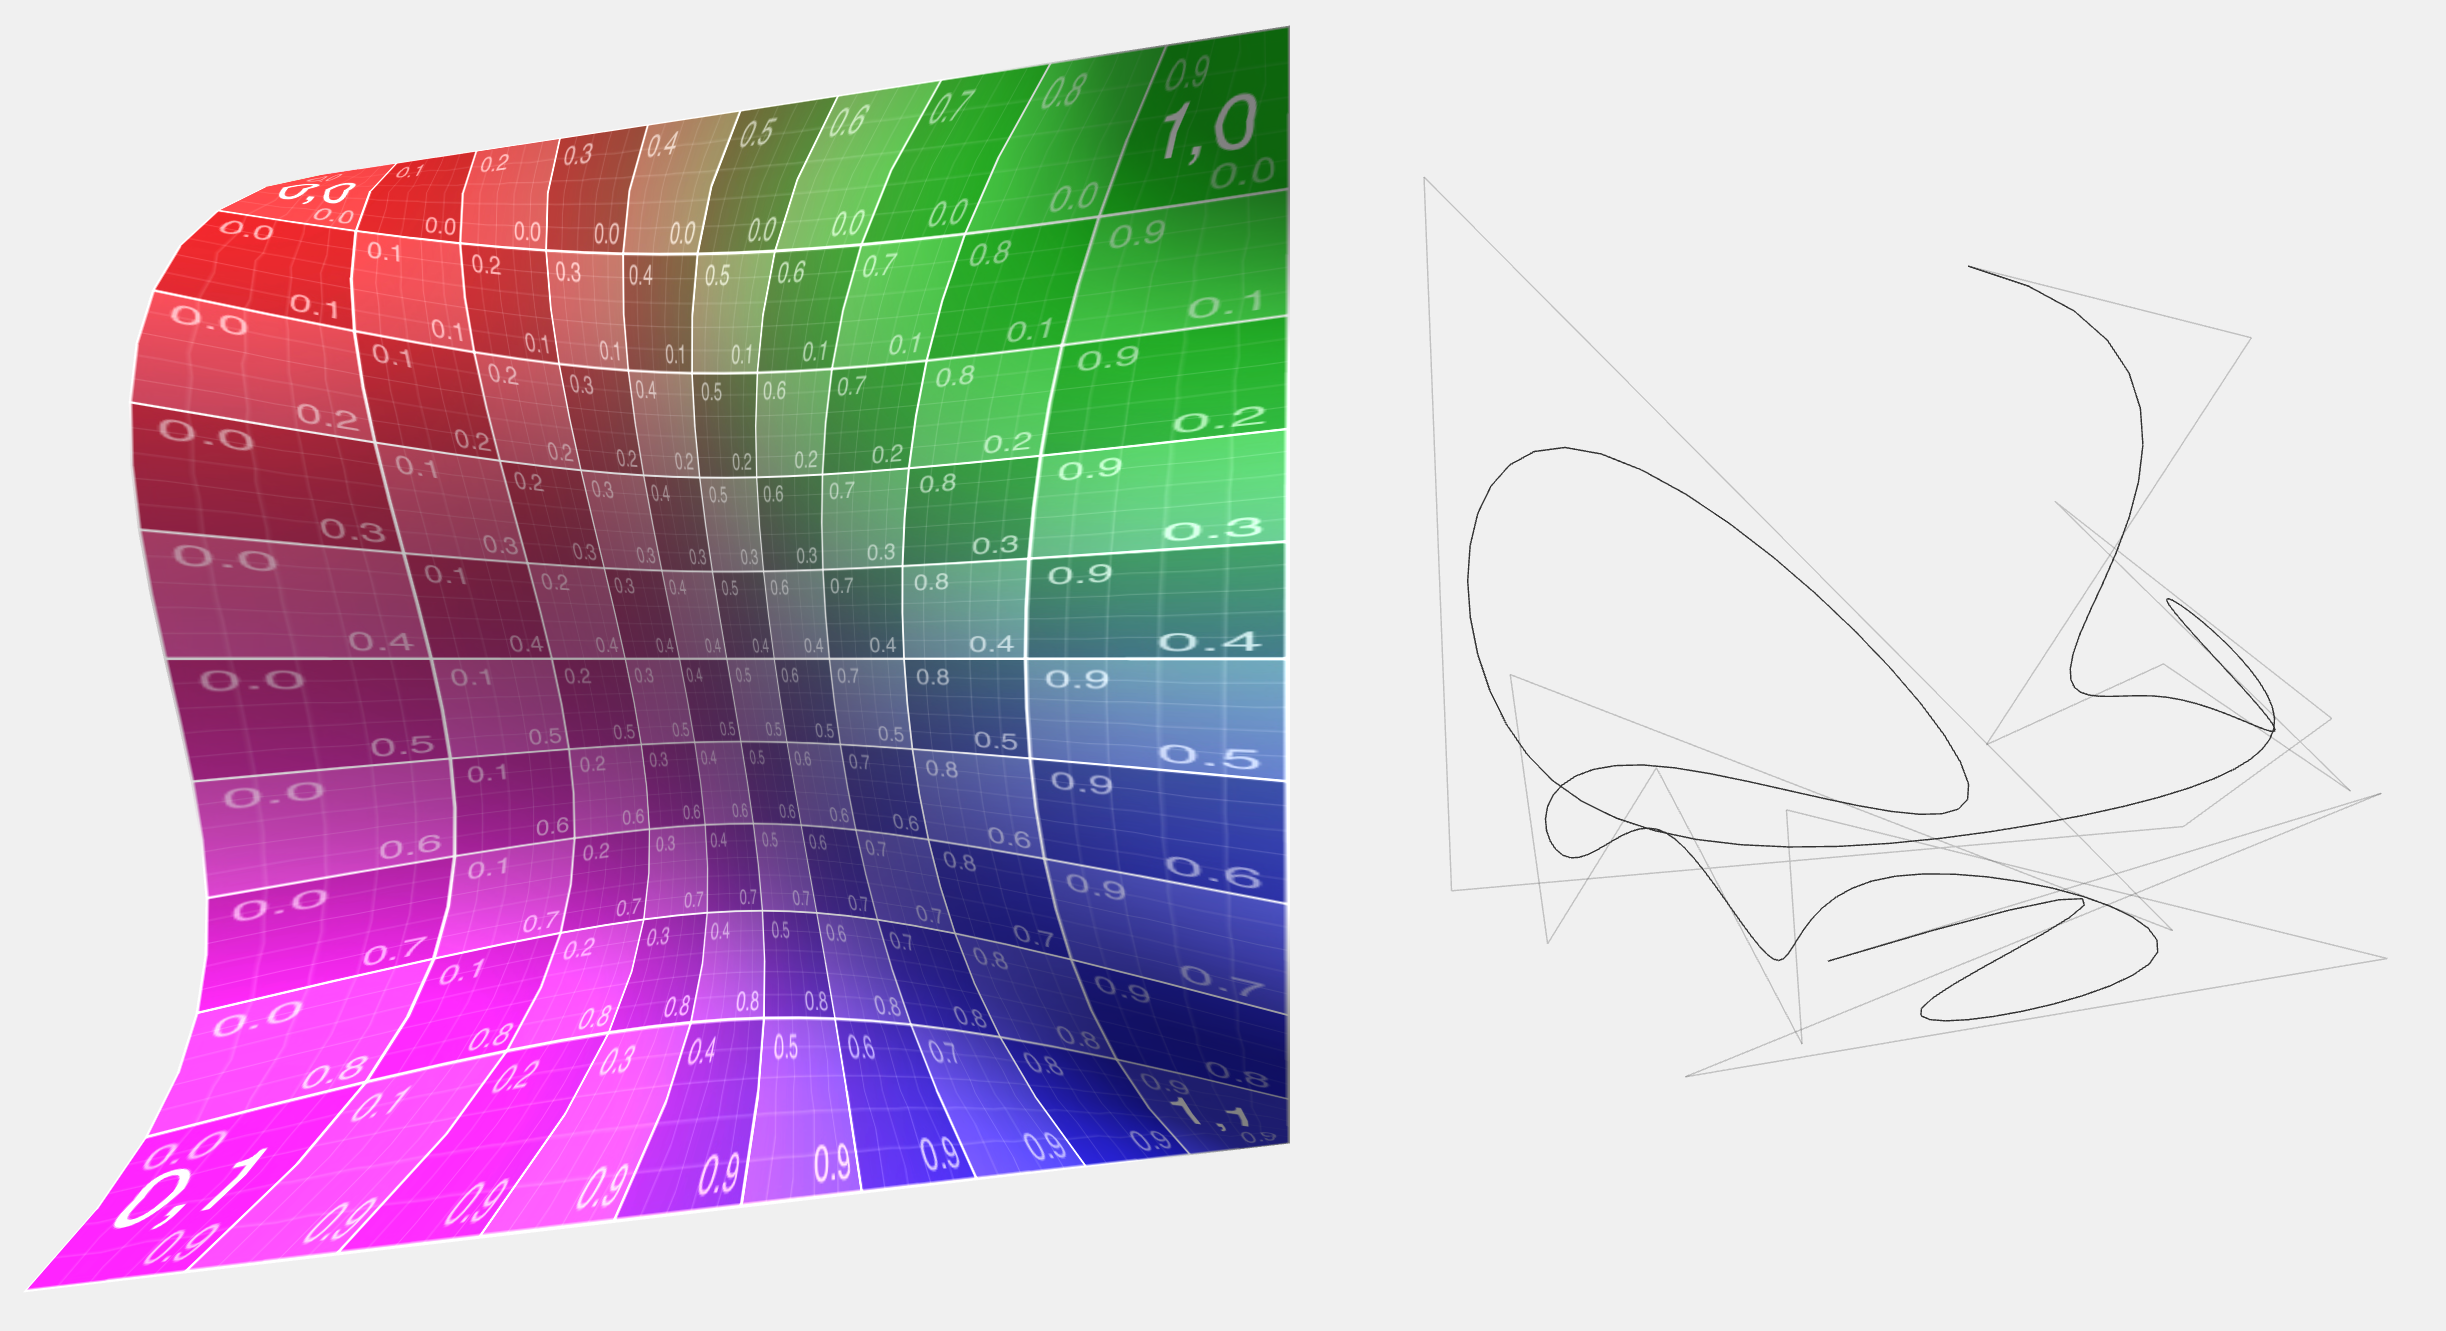
\includegraphics[width=\textwidth]{images/nurbs}}
					\caption{A screenshot of the NURBS curve and surface example.}
					\label{fig:nurbs}
				\end{figure}
		
			}
			
		}
		
		\newpage
		
		\section{Risk assessment} {
		\label{app:risk_assessment}
		
			\subsection{Category legend} {
			\label{app:category_legend}
			
				\begin{table}[H]
				\caption{A list of the categories used in the risk assessment.}
				\begin{tabularx}{\textwidth}{@{}lX@{}}
					\toprule
					\textbf{Risk category} & \textbf{Examples} \\
					\midrule
					Project management & Operational, organisational and contractual software development parameters. \\
					Process management & Planning, staffing, tracking, quality assurance and configuration management. \\
					Technical process & Analysis, design, programming and testing. \\
					Technical product & Requirements stability, design performance, code complexity and test specifications. \\
					\bottomrule
				\end{tabularx}
				\end{table}
			
			}
			
			\subsection{Strategy legend} {
			\label{app:strategy_legend}

				\begin{table}[H]
				\caption{A list of the risk strategies used in the risk assessment.}
				\begin{tabularx}{\textwidth}{@{}lX@{}}
					\toprule
					\textbf{Risk strategy} & \textbf{Description} \\
					\midrule
					Acceptance & The risk is acceptable and will be account for. \\
					Avoidance & An activity will not be performed if it may result in a risk. \\
					Reduction & The severity of the impact or the likelihood of the risk will be reduced. \\
					Research & The risk will be investigated so it can be managed. \\
					Transfer & The risk is shifted to or outsourced to another person, group or organisation. \\
					\bottomrule
				\end{tabularx}
				\end{table}

			}

			\subsection{Risk rating legend} {
			\label{app:risk_rating_legend}

				\begin{table}[H]
				\caption{The mapping between the priority score and its associated risk rating.}
				\begin{tabularx}{\textwidth}{@{}XX@{}}
					\toprule
					\textbf{Priority score} & \textbf{Risk rating} \\
					\midrule
					0 - 19 & Very low \\
					20 - 39 & Low \\
					40 - 59 & Medium \\
					60 - 79 & High \\
					80 - 100 & Very high \\
					\bottomrule
				\end{tabularx}
				\end{table}

			}
			
			\subsection{Risk details} {
			\label{app:risk_details}
			
				\begin{table}[H]
				\caption{The details of the risks that were outlined in Section~\ref{sec:risks}.}
				\begin{spreadtab}{{tabularx}{\textwidth}{@{}llXXXX@{}}}
					\toprule
					@\textbf{Id} & @\textbf{Category} & @\textbf{Likelhood} & @\textbf{Impact} & @\textbf{Score} & @\textbf{Rating} \\
					\midrule
					1 & @Project management & :={35}\% & 95 & (c2 / 100) * d2 & \rating{:={e2 * 100}} \\
					2 & @Technical product & :={10}\% & 80 & (c3 / 100) * d3 & \rating{:={e3 * 100}} \\
					3 & @Technical product & :={10}\% & 100 & (c4 / 100) * d4 & \rating{:={e4 * 100}} \\
					4 & @Technical product & :={60}\% & 100 & (c5 / 100) * d5 & \rating{:={e5 * 100}} \\
					5 & @Process management & :={5}\% & 85 & (c6 / 100) * d6 & \rating{:={e6 * 100}} \\
					6 & @Technical process & :={1}\% & 75 & (c7 / 100) * d7 & \rating{:={e7 * 100}} \\
					7 & @Technical product & :={20}\% & 85 & (c8 / 100) * d8 & \rating{:={e8 * 100}} \\
					8 & @Technical product & :={20}\% & 85 & (c9 / 100) * d9 & \rating{:={e9 * 100}} \\
					\bottomrule
				\end{spreadtab}
				\end{table}
			
			}
		
		}
		
	\end{appendices}
	
\end{document}
